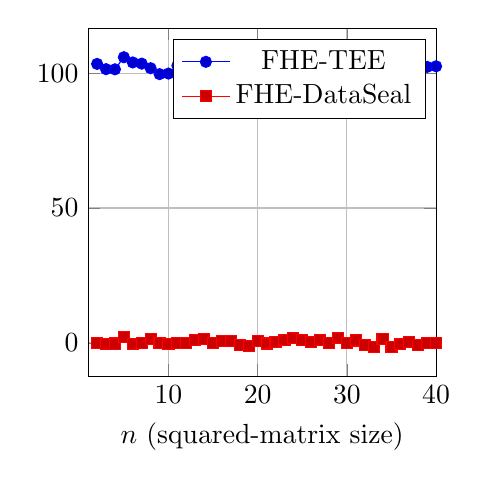
\begin{tikzpicture}
\begin{axis}[
    width=6cm, % Set the width of the plot to the text width of the subfigure
    height=6cm, % You can adjust the height as needed
    xlabel={$n$ (squared-matrix size)},
    % ylabel={Time in Seconds},
    legend pos=north east,
    grid=both,
    xmin=1, xmax=40,
    % ymin=0, ymax=20
]
\addplot table {
n	FHE-TEE
2	103.4056938
3	101.4611175
4	101.3920407
5	105.8879499
6	103.9500244
7	103.5089962
8	101.8246205
9	99.62424363
10	99.82276919
11	102.7803605
12	103.8931055
13	103.3746956
14	102.5331162
15	102.6862143
16	100.4000167
17	102.543188
18	100.3491737
19	100.4502277
20	100.7606704
21	103.5287395
22	102.3706782
23	103.2764584
24	104.02449
25	105.0851702
26	105.305407
27	103.138192
28	103.1277331
29	103.368338
30	103.466807
31	103.3426362
32	105.01379
33	96.78144641
34	101.0244141
35	99.84221011
36	101.2957559
37	100.8330264
38	103.4609148
39	102.3066773
40	102.5258032
};
\addlegendentry{FHE-TEE}

\addplot table {
n	vFHE
2	-0.1996514023
3	-0.3367357677
4	-0.2684274668
5	2.115318454
6	-0.2969423964
7	0.0346212436
8	1.361980986
9	0.06717432262
10	-0.3168196742
11	-0.1402666128
12	-0.1549811581
13	1.044269571
14	1.510851286
15	-0.1738512829
16	0.6107445017
17	0.8193890185
18	-0.7822330341
19	-1.021427895
20	0.654860921
21	-0.2497473425
22	0.3767789386
23	0.9448686042
24	1.876042098
25	1.147679864
26	0.3383018636
27	1.085888756
28	0.04266302609
29	1.794990649
30	-0.01382045108
31	0.8835936002
32	-0.9035748995
33	-1.416225604
34	1.371155153
35	-1.592052841
36	-0.3674215991
37	0.2815344946
38	-0.7478491415
39	-0.1308865844
40	-0.1820780183
};
\addlegendentry{FHE-DataSeal}



\end{axis}
\end{tikzpicture}


